\documentclass[11pt]{article}

\usepackage{fullpage}
\usepackage{amsmath}
\usepackage{epsfig}
\usepackage{graphics}
\usepackage{caption}
\usepackage{circuitikz}
\usepackage{enumitem}

\oddsidemargin -0.15in
\evensidemargin -0.15in
\headheight 0in
\headsep 0in
%\topmargin -0.25in
\textheight 9.3in
\textwidth 6.8in

\setlength\parindent{0pt}
\setlength\parskip{3mm}

\renewcommand\u[2][]{\ensuremath{\,\text{#2}^{#1}}}

\makeatletter
 \renewcommand\section{\@startsection {section}{1}{\z@}%
     {-2.5ex \@plus -1ex \@minus -.2ex}%
    %  {1.3ex \@plus.2ex}%
     {0.2ex \@plus.2ex}%
    {\bfseries\Large}}
     % {\centering\bfseries}}
\renewcommand\subsection{\@startsection {subsection}{2}{\z@}%
     {-2.5ex \@plus -1ex \@minus -.2ex}%
     {0.2ex \@plus.2ex}%
    {\bfseries\large}}
%% \@startsection {NAME}{LEVEL}{INDENT}{BEFORESKIP}{AFTERSKIP}{STYLE} 
%            optional * [ALTHEADING]{HEADING}
%    Generic command to start a section.  
%    NAME       : e.g., 'subsection'
%    LEVEL      : a number, denoting depth of section -- e.g., chapter=1,
%                 section = 2, etc.  A section number will be printed if
%                 and only if LEVEL gt or eq the value of the secnumdepth
%                 counter.
%    INDENT     : Indentation of heading from left margin
%    BEFORESKIP : Absolute value = skip to leave above the heading.  
%                 If negative, then paragraph indent of text following 
%                 heading is suppressed.
%    AFTERSKIP  : if positive, then skip to leave below heading,
%                       else - skip to leave to right of run-in heading.
%    STYLE      : commands to set style
%  If '*' missing, then increments the counter.  If it is present, then
%  there should be no [ALTHEADING] argument.  A sectioning command
%  is normally defined to \@startsection + its first six arguments.
\makeatother

\begin{document}


\begin{center}
\section*{
Franklin \& Marshall College \hfill PHY 223\\
\bigskip
{\Large \it Understanding Uncertainty}}
\end{center}

Numerical values in physics derive a lot of meaning from their associated
uncertainty. The speed of light, for example, was measured in 1972 to have a value of $\textrm{c} =
299,792,456.2 \pm 1.1$ m/s. That's an uncertainty on the order of 0.0000004\%!
Such accuracy is why we can use the speed of light to define other values, such
as the length of a meter (as long as we have a very accurate way to measure time as
well). If our best measurement of light had a 1\% error instead, we would not be
able to use it as a standard.

While this is an extreme example of the need for quoted uncertainty, every
experimentally determined value in physics must include a range of confidence in
other to be meaningful. If you measure a quantity of $x=47.3$ in the lab, the size
of the uncertainty can completely change its meaning. If $\delta x = 0.5$, then
the reported value is $x = 47.3 \pm 0.5$. If instead $\delta x = 934$, then the
reported value is $x = 0 \pm 900$. 

In many texts, scientists and engineers use the word error synonymously with
uncertainty, which can lead to confusion. Errors in measuring a quantity due to
not following procedures are not valid sources of uncertainty. ``Human error''
should never be part of your consideration. If a lab error does occur, you have
to redo the measurement. Uncertainty represents your level of confidence in a
value that was measured to the best of your ability limited by the equipment to 
which you have access.

\section{Error estimation vs. propagation}

The uncertainty for a value that you measure in the lab depends on the details
of the measurement. What is the accuracy of the measurement device? What 
environmental conditions are affecting your measurement? How can you
estimate (rigorously) the size of the uncertainty? For example, you might measure
the distance traveled by an object in the lab and how long it took. You would
have two individual measurements, distance and time, each with their own
uncertainty that would depend on how you measured them.

For derived values, you must \textit{propagate} one or more sources of uncertainty to
find the overall uncertainty. In the example above, consider that you want to
calculate the velocity of the object. How would you combine the uncertainty in
distance traveled and the uncertainty in how long it took?

It's important to distinguish between those two skills (estimation and
propagation) and we will cover them both below.

\section{Estimating uncertainty of a measurement}

There is an uncertainty involved in any measurement made in experimental work. 
The uncertainty can come in part from the inherent precision of the measurement 
device. This can often be calculated with great accuracy. Any 
research-grade piece of equipment will provide a complete characterization of 
the variability of the measurements. Beyond the equipment, variations (random or 
systematic) in experimental conditions can also contribute to uncertainty. These 
can be much harder to estimate and can involve a certain amount of educated 
guesswork. Eventually, the uncertainty provides \textit{the degree of confidence 
in the results of the measurement}.  

\subsection{Random vs. systematic error}

Imagine an experiment where we drop a ball from a tall building 20 times and we 
measure the position of the impact on the ground. We record our data on a target 
sheet of paper. If there is no wind, the ball will fall within a tight circle 
around the center of the target (as shown in figure 1a).

\begin{figure}[h]
\begin{center}
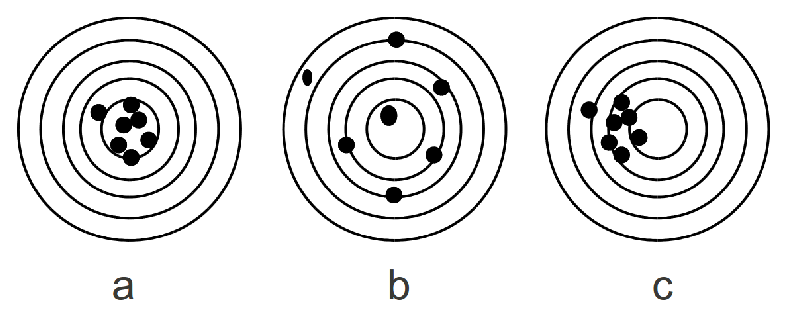
\includegraphics{Figure1.eps}
\caption{Example of impact positions showing (a) a small random error, (b) a 
larger random error, (c) a small random error and a non-zero systematic error.}
\end{center}
\end{figure}

The reason the balls do not all fall in the same spot can be many: irregularities in
the shape of the ball, vibrations in the initial device holding the ball, variable air 
currents as the ball falls, etc. All of these parameters are referred to as 
\textit{random errors}--they will be different in magnitude and direction each time you 
drop the ball in an unpredictable manner. In 
the case of figure 1(a), the random error would be considered relatively small. 
In the case shown in figure 1(b), it would be considered larger. In other words, 
random errors cause the data points (positions of the ball) to wander around the 
average position (the center of the target).

Systematic errors affect measurements in a different way. Imagine that in the 
example above, a breeze blows gently (but consistently) toward the left. All of the 
balls would drift in that direction by some amount. The target on the ground 
might look like figure 1(c).

Systematic errors can be found (and corrected for) by comparing a result to one 
known to be more reliable. Unfortunately, such known results often may not be available 
or may not even exist! Detecting systematic errors and estimating the uncertainty 
in a measurement due to systematic errors is usually very difficult.

\subsection{Precision of the measuring device}

When you use a device with a scale, such as a ruler, a graduated cylinder, or 
a speedometer, the precision of the scale is indicated by the distance between 
closest tick marks. With digital devices, like a stopwatch, the precision is 
indicated by the smallest decimal place. With any of these measuring devices, we 
usually estimate the associated uncertainty as half the smallest division. For a 
ruler with millimeter tick marks, then, the uncertainty in a length measurement 
made with that ruler would be $\pm$ 0.5 mm.

\subsection{Repeated measurements}

Often, however, the uncertainty in a measurement is not limited by the 
precision of measuring device, but by the procedure for measurement. Consider a 
researcher measuring the falling time of an object, using a stopwatch with 1 
millisecond precision. They repeat the measurement several times and collect the 
following data:

0.452 s, 0.488 s, 0.511 s, 0.443 s, 0.501 s, 0.526 s, 0.492 s, 0.550 s, 0.469 s, 
0.471 s

The researcher is measuring the same event, which presumably has a definite time 
duration, but there is greater variation in the measurement than the precision 
of the stopwatch (1 ms). This is likely due to the finite (and variable) reaction 
time of the researcher, which results in a random and/or systematic variation of 
the time values. 

When we measure something multiple times, we try to 
control the process so that it occurs in the same way every time. However, some 
things are outside our control, like the reaction time when using a stopwatch. 
\textbf{Random error often increases the uncertainty above the precision of the 
measuring device!} 

The best way to determine if there is random error that is larger than the 
precision of your measuring device is to perform the measurement several times
and use statistics to compute values. 

\textbf{\underline{Mean:}}

The mean is the average value of a set of numbers, and is what you will use for 
the best estimate of your measurement. For a set of N measured values, the mean 
is given by:
\begin{equation}
\overline{x} = \frac{x_{1}+x_{2}+x_{3}+\ldots +x_{N}}{N} = 
\frac{1}{N}\sum_{i=1}^{N} x_{i}
\label{eq:Mean}
\end{equation}
For example, the mean of the time measurements listed above is:
\begin{equation}
\nonumber \overline{x} = \frac{0.452\textrm{s} + 0.488\textrm{s} + 0.511\textrm{s} +  0.443\textrm{s} + 0.501\textrm{s} + 
0.526\textrm{s}  + 0.492\textrm{s} + 0.550\textrm{s} + 0.469\textrm{s} + 0.471\textrm{s}}{10} = 0.490\u{s}
\label{eq:MeanExample}
\end{equation}
 
\textbf{\underline{Gaussian distribution:}}

When most measurements are repeated a very large number of times we expect that 
half of the data will be $\geq$ the average and half will be $\leq$ the average. 
We also expect that most of the results will be fairly close to the average and 
a smaller number of results will be further from the average. When plotted in a 
histogram, data with random error will form a bell-shaped curve, known as a 
normal or Gaussian distribution. An example of a Gaussian distribution is shown 
in the figure below. 

\begin{figure}[h]
\begin{center}
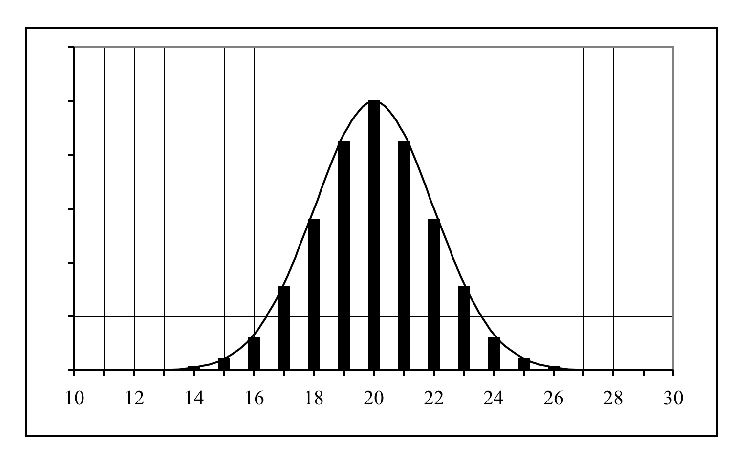
\includegraphics{Figure2.eps}
\caption{A histogram of measurements for a normal distribution with an average 
 $\bar{x}=20$ and a standard deviation $\sigma=2$.  The vertical axis represents
 the fraction of occurrences corresponding to each value on the horizontal axis. 
 Axis labels have been omitted to emphasize the general shape of the distribution.}
\end{center}
\end{figure}

\textbf{\underline{Standard deviation:}}

The uncertainty in a large number of measurements with random error is defined 
by the standard deviation, denoted as $\sigma$. The formal mathematical 
definition of the standard deviation\footnote{Technically, this formula gives the \textit{sample} standard deviation. To learn more about it (and why there is a $N-1$ instead of $N$ on the bottom of the formula), talk to your instructor or take PHY 322: Data Analysis \& Visualization.} is:
\begin{equation}
\sigma = \sqrt{\frac{\sum_{i=1}^{N}\left(x_{i}-\overline{x}\right)^{2}}{N-1}}
\label{eq:Std}
\end{equation}
where $\overline{x}$ (given in equation \ref{eq:Mean}) is the mean and N is the 
number of measurements ($x_{i}$). However, in lab you will most often use Python 
or other mathematical software to do the calculation for you.

An intuitive way to understand the standard deviation is that about 2/3 of the 
measurements will have a value that falls within the range: ($\bar{x}\pm\sigma$), about 95$\%$ of the data fall within the range: $(\bar{x}\pm 
2\sigma)$, and more than 99$\%$ of the data fall within the range: ($\bar{x}\pm 3\sigma$).

The standard deviation of the time measurement values above is $0.033\,$s. Note 
that all the values fall within the $2\sigma$ range: $0.42\u{s} - 0.56\u{s}$, and most 
of the values fall within the $1\sigma$ range: $0.46\u{s} - 0.52\u{s}$.

\subsection{Counting experiments}

Some experiments involve counting how many time a specific event occurs. For
example, in a radioactive decay such as gamma spectroscopy, we'll count how many
times a gamma photon was detected with a specific energy. In those cases, if you
detect $N$ events, the uncertainty is $\sqrt{N}$. In other words, if you detect
100 events in a 2-second window, you would expect the next 2-second window to
have $100\pm\sqrt{100}=100\pm10$ counts in it---that is, somewhere between 90 and 110 counts.

This value of $\sqrt{N}$ can be derived, but that is beyond the scope\footnote{To
learn more about it, talk to your instructor or take PHY 322: Data Analysis \& Visualization.}
of this document. However, we can see that while the absolute size of the uncertainty
will grow as $N$ increases, the \textit{fractional} uncertainty 
$\sqrt{N}/N = 1/\sqrt{N}$ will decrease, indicating that larger measurement are more precise 
relative to their scale.
For example, a repeated experiment that yields 10 events on average will generate 
$10\pm\sqrt{10}\approx10\pm3$ events each time the experiment is conducted (a 30\% uncertainty), 
whereas a much longer experiment that yields 1000 events on average will generate
$1000\pm30$ events for each iteration (a 3\% uncertainty).

\subsection{Reporting uncertainty}

\subsubsection{Standard Form}
\textit{You should always report uncertainty for any measurement.} There is a 
\textbf{standard form} for reporting uncertainty:
\begin{equation}
(x \pm \delta x)\u{[units]}
\end{equation}
In this statement, $x$ is the measured value and $\delta x$ is its uncertainty. 
For example, if you measure the diameter of a marble to be $15.2\u{mm}$ with an 
uncertainty of $0.5\u{mm}$, you would express this in standard form as:
\begin{equation}
(15.2 \pm 0.5)\u{mm}
\end{equation}

\textbf{Notice that both the measurement and the uncertainty have units!} This 
standard form actually expresses a \textbf{range} of length values. The diameter 
of the marble falls somewhere within the range of $14.9\u{mm}$ to $15.7\u{mm}$.

\subsubsection{Rounding and Significant figures}

In physics, we follow two simple rules for rounding:
\begin{enumerate}
\item Round the uncertainty to \textbf{one}\footnote{In certain cases two significant figures may be appropriate for the uncertainty---talk to your instructor if you want to discuss. One digit is a good rule of thumb, however.} significant figure.
\item Round the measured value to the \textbf{same decimal place} as the 
uncertainty.
\end{enumerate}

For example, if you measured the size of an object several times and found the following 
values for mean and standard deviation:

Mean: $L = 0.54682\u{m}$

St. Dev: $\delta L = 0.038216\u{m}$

You would round as follows: First, the standard deviation to one sig fig: 
$\delta L = 0.04\u{m}$, and second, the mean to the same decimal place: $L = 0.55\u{m}$. In standard form:

$L = (0.55 \pm 0.04)\u{m}$

\textbf{BE CAREFUL} not to round all the numbers before you propagate the 
uncertainty. It is okay to have too many significant figures during 
intermediate steps in your calculation. Only a value that will be reported as 
collected data or a final result should be rounded. If you round your values too 
early, you will introduce additional mathematical errors into your calculation.

\subsection{Exercises:}

\begin{enumerate}
\item Write the following quantities in their final reporting form:
  \begin{enumerate}
  \item 341.222 m with an uncertainty of 0.345 m.
  \item 341.222 m with an uncertainty of 10.345 m.
  \item $1.2395\times10^{-2}\,$s $\pm$ $4.452\times10^{-4}\,$s.
  \item $4.640\times10^2\,$m/s with an uncertainty of $3.495\times10^5\,$m/s.
  \end{enumerate}

\item If you measure radioactive counts in the lab and record 5391 of them. What
  is the uncertainty in this value? How would you report this number?

\item You make 10 time measurements and get 5.6, 5.5, 5.2, 5.5, 5.8, 6.0, 5.8,
  5.1, 5.3, 5.8. How should you report your measurement of the time? %Assume that the precision
  %of each measurement is on the order of 0.005 seconds and can be ignored given
  %larger sources of uncertainty.
\end{enumerate}

\section{Propagating uncertainty}

In many experiments, you will use measured quantities to calculate values of
interest. For example, imagine that you are trying to calculate the
gravitational acceleration near the Earth's surface $g$ from your observations
of a pendulum:

\begin{equation}
 g = \frac{4\pi^2L}{T^2}
 \label{eq: g from pendulum}
\end{equation}

where $L$ is the length of the pendulum and $T$ is the period of oscillation.
The respective uncertainties for these values are $\delta L$ and $\delta T$.
What is the uncertainty $\delta g$?

\subsection{Partial derivative method}

You will have previously encountered simple rules for error propagation. Those
rules tend to overestimate the size of the error, and they can be hard to implement 
when your result is a complicated function of your measured variables. A better general 
rule can be calculated from the mathematical relationship between the derived quantity 
and the measured values.

Consider a value $z$ derived from an arbitrary number of values with uncertainty 
$(x_{i} \pm \delta x_{i})$ through a function:
\begin{equation}
  z = f(x_{0},\, x_{1},\, x_{2},\, \ldots)
\end{equation}

As long as the different values $x_i$ that we measured are \textit{independent} of each other, 
we can determine the uncertainty on $z$ from the following general formula:

\begin{equation}
  \boxed{\delta z^{2} = \left(\frac{\partial f}{\partial x_{0}}\right)^{2}\delta 
    x_{0}^{2} + \left(\frac{\partial f}{\partial x_{1}}\right)^{2}\delta x_{1}^{2} 
    + \left(\frac{\partial f}{\partial x_{2}}\right)^{2}\delta x_{2}^{2} +  \ldots}
\end{equation}

Another way of saying this is that the square of our total uncertainty in $z$ will be a sum of several terms, each of which depends on (1) the uncertainty on the measurement $x_i$, and (2) the partial derivative of the function that determies $z$ with respect to $x_i$.

In our example above, our measured values (the $x_i$'s) are $L\pm\delta L$ and $T\pm\delta T$, and our derived quantity is $g$, so we can calculate the contributions to the uncertainty on $g$ from both $L$ and $T$:

\begin{equation}
  \frac{\partial g}{\partial L} = \frac{4\pi^2}{T^2}
\end{equation}

and

\begin{equation}
  \frac{\partial g}{\partial T} = -\frac{8\pi^2 L}{T^3}\quad
\end{equation}

such that

% \begin{eqnarray}
%   \delta g &=& \sqrt{\left( \frac{\partial g}{\partial L} \right)^2\delta L^2
%                  + \left( \frac{\partial g}{\partial T} \right)^2\delta T^2}\\
%              &=& \sqrt{\left( \frac{4\pi^2}{T^2} \right)^2 \delta L^2+
%                  \left( -\frac{8\pi^2L}{T^3} \right)^2\delta T^2}%\\
%             %  &=& \ldots \nonumber
% \end{eqnarray}

\begin{eqnarray}
  \delta g &=& \sqrt{\left( \frac{\partial g}{\partial L} \right)^2\delta L^2
                 + \left( \frac{\partial g}{\partial T} \right)^2\delta T^2}=\sqrt{\left( \frac{4\pi^2}{T^2} \right)^2 \delta L^2+
                 \left( -\frac{8\pi^2L}{T^3} \right)^2\delta T^2}
\end{eqnarray}


\subsection{Introduction to (review of) partial derivatives}

You will learn about partial derivatives in your math courses. For the purpose
of this course, we will only cover some very basic notions. Consider the
following function

\begin{equation}
f(x, y, z) = 3x + x^2y + xyz
\end{equation}

If we take the partial derivative of $f$ with respect to $x$, we are looking at
the rate of change of $f$ when $x$ changes but both $y$ and $z$ do not change.
Mechanically, you can take the derivative with respect to $x$ assuming that $y$
and $z$ are constants. We use a specific symbol to indicate that we are taking
a partial derivative:

\begin{equation}
\frac{\partial f}{\partial x} = 3 + 2xy + yz
\end{equation}

\begin{equation}
\frac{\partial f}{\partial y} = x^2 + xz
\end{equation}

\begin{equation}
  \frac{\partial f}{\partial z} = xy
\end{equation}

We can also take a second derivative, which can be with respect to the same variable or not:

\begin{equation}
  \frac{\partial^2 f}{\partial x^2} = 2y
\end{equation}

\begin{equation}
  \frac{\partial^2 f}{\partial x \partial y} = \frac{\partial^2 f}{\partial y \partial x}
  = 2x+z
\end{equation}

and so on.

\subsection{Exercises:}

\begin{enumerate}[resume]

\item Consider the following function: $f(x, y, z) = y^x + \cos(2\pi z/L_z)$.
  What are:
  \begin{enumerate}
  \item $\partial f/\partial x$?
  \item $\partial f/\partial y$?
  \item $\partial f/\partial z$?
  \item $\partial^2 f/(\partial x\partial y)$?
  \end{enumerate}

\item Consider calculating the speed of an object by measuring the distance it
  travels and the time it took to do it. You get a distance of $L = 1.30 \pm
  0.05$ m and a time of $t = 0.43 \pm 0.02$ s.
  \begin{enumerate}
  \item Using the partial derivative method, write the equation for the
    uncertainty in speed.
  \item Calculate the speed with uncertainty. Make sure to properly format
    your answer.
  \end{enumerate}

\item If you measure the radioactive counts of a sample in the lab and record
  8100 events in a time $t = 12.8 \pm 0.3\u{s}$. What is the count rate (in counts/s), including
  uncertainty? 
\end{enumerate}

\section{Data fitting}

A powerful tool to compare your data to existing models and theories is curve
fitting, where you can check how well your measurements (or derived values)
match know functions. In this course, we will not derive the algorithms for data
fitting\footnote{To learn more about data fitting methods, talk to your instructor 
or (you guessed it) take PHY 322: Data Analysis \& Visualization.}. We will however 
learn how to use those tools effectively.

\subsection{Residuals, RMSE, $\chi^2$, and R$^2$ values}

Whenever you attempt to fit a function to a data set, the software you use will
return a value indicating how closely it was able to match the function. There
are multiple options that have subtle but important differences. Here will look
at a few common ways of describing this agreement:
\begin{itemize}
\item {\bf Residuals.} The \textit{residuals} of the data are the differences between the
 measured values and the values predicted by the model:
 \begin{equation}
  \Delta x_i = x_i-\hat{x}_i
\end{equation}
where $\Delta x_i$ is the residual, $x_i$ represents the data point, and $\hat{x}_i$ is the expected value
calculated from the model function. %The residuals also have \textbf{the same units as the data}. 
When calculating residuals, you will end up with one value 
for each of the points in your dataset: some of them will be positive, some will be negative, 
some may be large (in magnitude) and others may be small. 
% If our measurements have uncertainties, it is useful to compare the residual of each measurement to the uncertainty on our corresponding point---if the magnitude of the residual is much larger than the uncertainty, then that may suggest the point is inconsistent with the model.

The residuals thus represent how well \textit{each individual 
point} agrees with the model. However, it is often useful to calculate a single value that describes
the agreement between the model and the dataset \textit{as a whole}. This is the reason for the
three other quantities described below.

\item {\bf Root-mean-square error (RMSE).} This quantity is calculated by squaring all the
 residuals, taking the mean, and then finally taking the square root:
\begin{equation}
  \textrm{RMSE} = \sqrt{\frac{\sum_i^N (x_i-\hat{x}_i)^2}{N}}= \sqrt{\frac{\sum_i^N \Delta x_i^2}{N}}
\end{equation}
where here again $x_i$ represents the data point and $\hat{x}_i$ is the expected value
from the model. You should notice that this formula is very similar to that for the standard deviation: the RMSE is effectively measuring \textit{the size of the scatter of the data about the model}. In the case of a good fit, the residuals should be small and 
\textbf{the RMSE value should be low.} %Note also that that the RSME has \textbf{the same units as the data}, since it is related to the average magnitude of the residuals. This also means the RMSE should be similar to the typical uncertainties (even though the uncertainties are not used in calculating the RMSE).

\item {\bf $\boldsymbol{\chi}^2$ value.} This quantity (pronounced ``KAI-square'') is also 
calculated from the residuals, but each residual is divided by its uncertainty before being 
squared and summed:
\begin{equation}
  \chi^2 = \sum_i^N \left(\frac{x_i-\hat{x}_i}{\delta x_i}\right)^2= \sum_i^N \left(\frac{\Delta x_i}{\delta x_i}\right)^2
\end{equation}
where $\delta x_i$ is the uncertainty on $x_i$ and the other variables are defined as above. Notice that 
both the RMSE and $\chi^2$ grow when the residuals are large (i.e., when the data is very different from the model), but $\chi^2$ accounts for the fact that large residuals are expected if the uncertainties are also large. In the case of a good fit, we expect $\Delta x_i\approx\delta x_i$ on average, which means {\bf the $\boldsymbol{\chi}^2$ value should be close to \textbf{\textit{N}}, the 
number of data points.} It is also common to report the \textbf{reduced $\boldsymbol{\chi}^2$}, defined as $\chi^2/N$, so a good model will have a reduced $\chi^2\sim1$. %Finally, since both $\Delta x_i$ and $\delta x_i$ have the units of the data, \textbf{$\boldsymbol{\chi}^2$ is unitless}.

\item {\bf R$^2$ value,} also called the coefficient of determination:
\begin{equation}
  R^2 = 1-\frac{\sum_i^N (x_i-\hat{x}_i)^2}{\sum_i^N (x_i-\bar{x})^2} = 1-\frac{\sum_i^N \Delta x_i^2}{\sum_i^N (x_i-\bar{x})^2}
\end{equation}
where $\bar{x}$ is the mean of the $x_i$ values and other values are defined as above. 
The $R^2$ value tells us the fraction of the total variation in the data explained by
the model: {\bf a good fit will have a value of R$^2$ that approaches 1}. \textit{We will not often use the $R^2$
value in our analysis, but we include it here for comparison to the other quantities since it is often used by other disciplines.}
\end{itemize}

\subsection{Best practices}

Curve fitting is useful to test whether certain models or equations fit your
data. It should generally {\bf not} be used to randomly guess a functional dependence.
Simply optimizing the values of the RMSE or $\chi^2$ do not always result in more
meaningful physical results, only formally-better fits. While physics uses the language
of math, not all math is physics. It is likely that you could fit a 20$^{th}$
order polynomial to most data sets, or even a 30$^{th}$ polynomial. The RMSE
would could be made infinitesimally small in these cases, but the results would 
be meaningless.

Below is a practical example. Imagine that you have a set of data that
corresponds to a cosine function around 0. If you don't know anything about the
functional form of your model, you might guess that a second order polynomial would 
provide a pretty good fit.

\begin{minipage}{\linewidth}
  \centering
  % 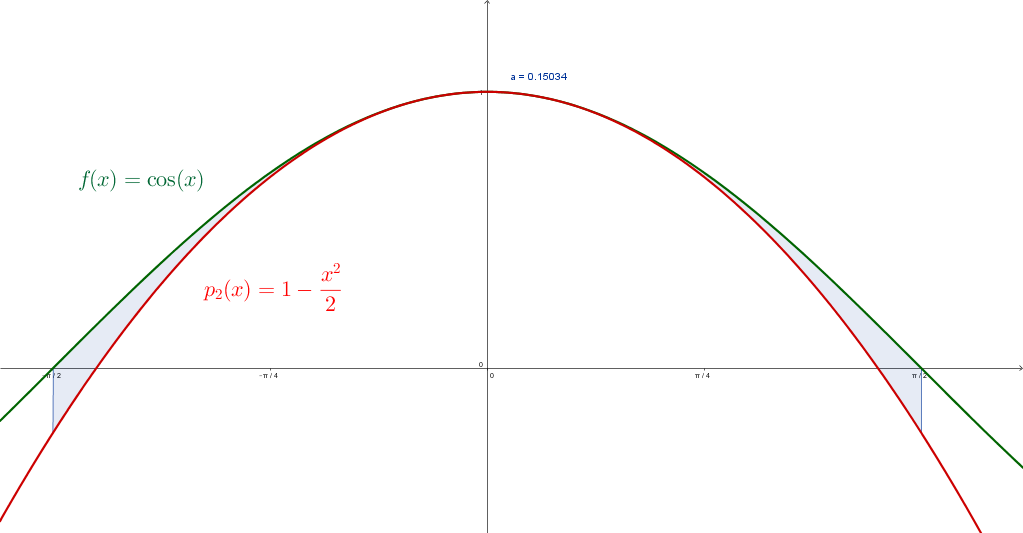
\includegraphics[scale=1.0]{./fitting.png}
  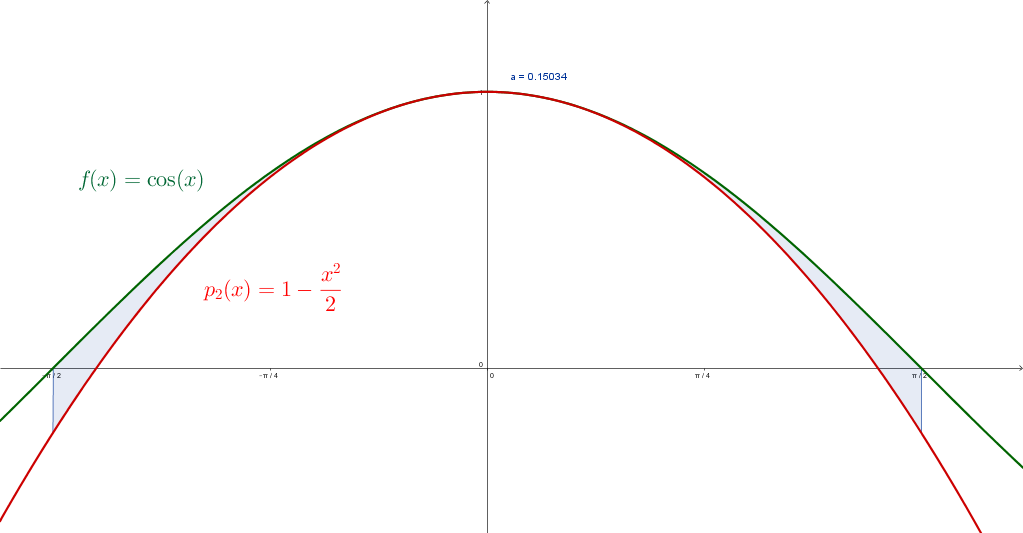
\includegraphics[width=8cm]{fitting.png}
  \captionof{figure}{Cosine (green) and quadratic (red) functions around the
    origin.}
  \label{fig fitting}
\end{minipage}

If you try the quadratic function and find it is not a good enough fit, you might be tempted to consider a quartic ($4^\textrm{th}$ order) function or even higher-order polynomials, which would inevitably give better fits. However, it would
be far better to consider the \textit{physics} of the problem, which might tell you that a cosine function is likely 
to describe the process giving rise to your data.

\subsection{Uncertainty}

Most often, you will use curve fitting with data that includes uncertainty. This
brings in two important consideration:

\begin{itemize}
\item You should always record the uncertainty in your fit parameters. For a 
physical model, the fit parameters (slope, period, acceleration, etc.) are often
the properties of the system we are trying to measure, so our final determination
of these values should be reported along with their uncertainties.
\item You should always use weighted fits (e.g., by finding the parameter 
  values that minimize the $\chi^2$ value, rather than the RMSE) when possible. 
  This kind of curve fitting weights data points with less uncertainty more heavily,
  so that data points with higher uncertainty do not affect the fit parameters as much.
\end{itemize}

\subsection{Exercises:}

 Consider a dataset consisting of the ($x$, $y$) values shown in the following table and plot. The plot also shows a linear model for the data, the equation for which is given below.\\

\begin{minipage}{0.4\textwidth}
  \vspace{0pt}
  
\begin{center}
\textbf{Data:}\vspace{2mm}\\
  \begin{tabular}{c|c}
  \textbf{$x$} & \textbf{$y$} \\\hline
  0.8 & $0.9\pm0.2$ \\
  2.7 & $1.6\pm0.2$ \\
  3.9 & $2.5\pm0.2$ \\
  4.8 & $2.6\pm0.2$
\end{tabular}
\vspace{1cm}

\textbf{Model:}
\vspace{-3mm}
  \[
f(x) = 0.4x+0.6
\]
\end{center}
\end{minipage}
\begin{minipage}{0.5\textwidth}
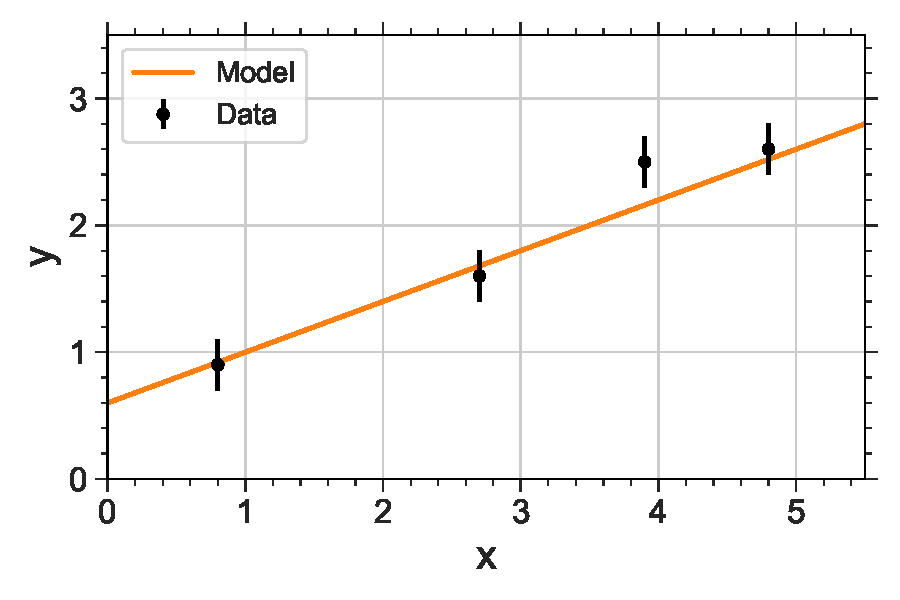
\includegraphics[width=\textwidth]{errorbar-graph.pdf}
\end{minipage}
\begin{enumerate}[resume]
\item Calculate the residuals to the model for each of the ($x$, $y$) pairs. Compare your results to the plot. How can you tell from the plot which points will have positive or negative residuals?
\vspace{4mm}
\item \begin{enumerate}
\item What is the RMSE for these data, given the model?
\item What is the $\chi^2$ value for these data, given the model?
% \item What is the $R^2$ value for these data, given the model?
\end{enumerate}\vspace{4mm}
\item In the plot we can see that the model overlaps with most of the error bars, but there is one point that does not overlap. Is this surprising? Would we expect a good model to overlap with all of the error bars? Explain why or why not.

\end{enumerate}
\end{document}
